\section{Data Processing}
\label{sec:data_processing}
\begin{comment}
Raw data was taken from STK, analysed and sorted in Matlab before trend analysis was carried out in Excel.

\subsection{Initial Sorting}
\end{comment}
The raw per-satellite data from STK was combined to create a data set representative of the performance of the constellation in question. A sample of the output from Matlab is given in Table \ref{tab:results_matlab}, with start and stop times given in fraction of days since January 1st, 1990. This sample was taken from the LAX-Heathrow flight simulation with reference case constellation of satellites. It shows rows demonstrating overlapping access times and the resulting calculations.

Rows of access times for all satellites were sorted by access start time. The difference between the access start time of the current row and the access stop time of the previous row was used to calculate the 'gap' time between accesses. In the case of overlapping access times, the difference is negative and discarded (marked in Table \ref{tab:results_matlab} as `N/A'). For these cases, the total `access time' is calculated as the difference between the end of the last calculated gap and the beginning of the current gap. 
% Table generated by Excel2LaTeX from sheet 'Sheet4'
\begin{table}[htbp]
  \centering
  \caption{Calculated access times from Matlab}
    \begin{tabular}{rrrrrrrr}
    \toprule
    Satellite & Access & Access Start & Access  Stop & Access & Gap Start & Gap Stop & Gap \vspace{-3mm} \\
    
    Number & Number & Time & Time & Length (s) & Time & Time & Length(s)\\
    \midrule
    2     & 6     & 41611.38 & 41611.39 & 845.73 & 41611.37 & 41611.38 & 664.42 \\
    1     & 6     & 41611.40 & 41611.41 & N/A  & 41611.39 & 41611.40 & 711.17 \\
    8     & 1     & 41611.41 & 41611.41 & 891.41 & N/A  & N/A  & N/A \\
    4     & 6     & 41611.42 & 41611.43 & N/A  & 41611.41 & 41611.42 & 676.12 \\
    7     & 1     & 41611.42 & 41611.43 & 895.24 & N/A  & N/A  & N/A \\
    3     & 6     & 41611.44 & 41611.44 & N/A  & 41611.43 & 41611.44 & 681.03 \\
    6     & 1     & 41611.44 & 41611.45 & 848.90 & N/A  & N/A  & N/A \\
    2     & 7     & 41611.45 & 41611.46 & N/A  & 41611.45 & 41611.45 & 697.37 \\
    5     & 1     & 41611.45 & 41611.46 & 936.46 & N/A  & N/A  & N/A \\
    1     & 7     & 41611.47 & 41611.48 & N/A  & 41611.46 & 41611.47 & 560.17\\
    \bottomrule
    \end{tabular}%
  \label{tab:results_matlab}%
\end{table}%

\subsection{Statistical Modelling} \label{sec:prob_distro}
The periodicity of concatenated access periods (discarding `N/A' values) was indicative of the number of `discrete' sample points available along a flight. A lower average period of access meant a higher access and update rate for a particular flight path. This higher effective sample rate would allow for potential deviations from a flight path to be detected earlier and with greater resolution.
\begin{comment} 
This is illustrated in Figure \ref{fig:periodicity}.
\begin{figure}[htbp]
	\centering
	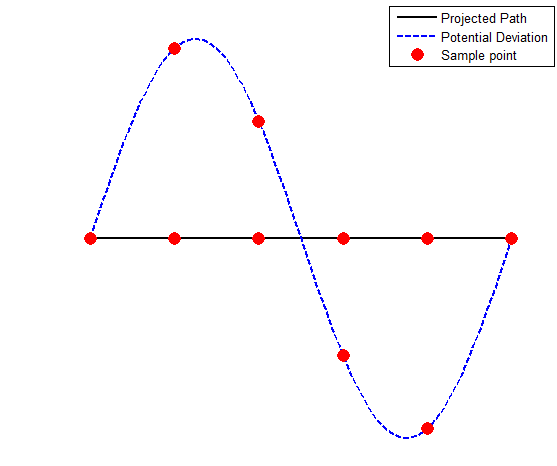
\includegraphics[scale = 0.7]{Pictures/periodicity.png}
	
	\caption{Diagram illustrating how a higher sample rate can detect flight path deviations}
	\label{fig:periodicity}
\end{figure} 
\end{comment}
The access periods for each flight and each constellation were analysed statistically by finding the statistical  model of best fit. This was achieved using the \verb|allfitdist| tool from \cite{sheppard12}. An example of the fitted distribution is given in Figure \ref{fig:allfitdist_Narita}. From the `best fit' model, the mean and standard deviation of the periods were extracted for consideration in the decision matrix.
\begin{figure}[htbp]
	\centering
	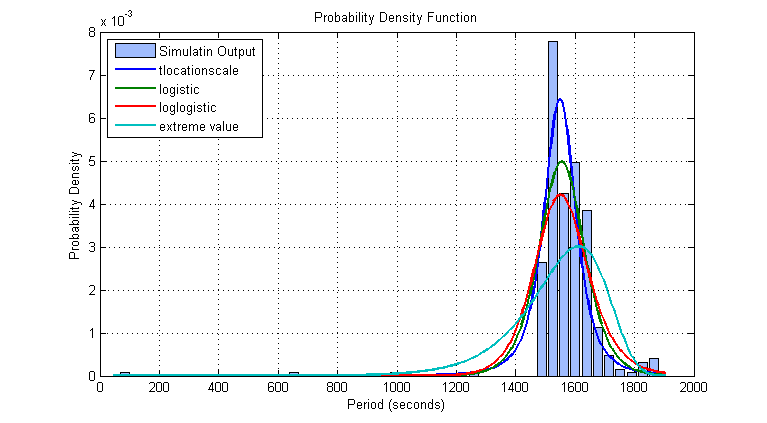
\includegraphics[scale = 0.75]{Pictures/allfitdist_Narita.png}
	
	\caption{Output of allfitdist when applied to the access periods of the LAX-Narita flight using the reference constellation described in Section \ref{sec:ref_case}}
	\label{fig:allfitdist_Narita}
\end{figure} 